\chapter{Technical background}
In this chapter we shall provide a technical background of the concepts which the protocol depends on. In addition, origins and implementations of those concepts will be described and related to the protocol and reference implementation work. The specific dependencies of the reference implementation, Ethereum and Docker, are also described.

\section{Bitcoin and the blockchain}
Bitcoin sparked a revolution in digital currencies when the white paper was released in 2009. The innovation of the blockchain and its implications is of special interest. All technical details are taken from the Bitcoin white paper \cite{btc}, unless noted otherwise.

\subsection{General idea}
The purpose of Bitcoin is to provide a financial system where participants can send and receive money without involvement of third parties. Traditionally, these third parties consist of a governmental institution controlling a currency, and one or more commercial banks that transfer money from the sender to the recipient. This is problematic because a third party can perform malicious actions and moreover exert complete control over the process. Bitcoin introduces a decentralized exchange of digital tokens, where no middleman is required, nor is any trust between sender and recipient required. The only requirement to use Bitcoin is to have a computer with Internet access. Bitcoin ownership is linked to cryptographic keys, thus, a cryptographic public key is analogous to a bank account number. The intrinsic value of Bitcoin is discussed in \cite{buterin:2011}. We shall now briefly discuss the key points of the Bitcoin whitepaper which enables the network to function. Below, Bitcoin (capitalized) refers to the Bitcoin network, whilst BTC refers to the currency.

\subsection{Transactions}
Transactions in the Bitcoin network are made in the following way: If Alice has one BTC and wants to send it to Bob, she will create a transaction stating that she transfers one BTC to Bob. The transaction is signed using her cryptographic private key, and then broadcast to the network. An attacker cannot spend Alice's BTC because the transaction can only be signed by Alice.

\subsection{Blockchain}
Bitcoin is based on the innovation called the ``blockchain''. Bitcoin nodes collect new transactions that are broadcast to the network, transactions are then checked for validity and placed together in a block of transactions. Besides the transactions, each of these blocks contain the hash of their parent block, and a nonce proving that sufficient work has been performed by the node creating the block. Since any valid transaction is part of some block, and all valid blocks are chained together, the blockchain can be seen as a distributed ledger, providing accountability. 

A new block is created approximately every 10 minutes. To calculate the current state of the network, the whole graph of blocks must be traversed.

\begin{figure}[ht]
\centering
\begin{tikzpicture}[auto] 
       \node[draw=none,text width=3cm] (block1) {Block};
       \draw[draw=black] (block1.north west) rectangle +(4.1cm, -2.25cm);
       \node[rectangle,draw] (hash1) 
            [below right=0.75cm and 0.15cm of block1.west,anchor=west] {Prev hash};
       \node[rectangle,draw] (nonce1) [right=0.3cm of hash1,anchor=west] {Nonce};
       \node[rectangle,draw] (item11) [below=0.8cm of hash1.west, anchor=west] {Tx}; 
       \node[rectangle,draw] (item12) [right=0.3cm of item11] {Tx};
       \node[rectangle,draw,minimum height=1.3em] (item12) [right=0.3cm of item12] {...};
       
       \node[draw=none,text width=3cm] (block2) [right=2cm of block1] {Block};
       \draw[draw=black] (block2.north west) rectangle +(4.1cm, -2.25cm);
       \node[rectangle,draw] (hash2) 
            [below right=0.75cm and 0.15cm of block2.west,anchor=west] {Prev hash};
       \node[rectangle,draw] (nonce2) [right=0.3cm of hash2,anchor=west] {Nonce};
       \node[rectangle,draw] (item21) [below=0.8cm of hash2.west, anchor=west] {Tx}; 
       \node[rectangle,draw] (item22) [right=0.3cm of item21] {Tx};
       \node[rectangle,draw,minimum height=1.3em] (item22) [right=0.3cm of item22] {...};

    \node[draw=none] (start1) [left=1.3cm of hash1] {\dots};
    \coordinate[right=0.2cm of nonce1] (start2);
    \coordinate[right=0.2cm of nonce2] (start3);
    \node[draw=none] (end) [right=1.4cm of nonce2] {\dots};
    \path[-latex] (start1) edge (hash1);
    \path[-latex] (start2) edge (hash2);
    \path[-latex] (start3) edge (end);
\end{tikzpicture}
\caption{Visualisation of blocks in the blockchain}
\end{figure}

\subsection{Proof-of-work}
As stated above the nonce is used to show that a node has performed a specific amount of work. This is done by calculating the hash of all the contents in the block, this hash has to adhere to the networks current difficulty level, which is a mechanic for controlling how long the network has to work before a block is found. Once every week the difficulty is adjusted, to the computational power in the network, to ensure an average block rate of approximately one every 10 minutes. There is no way to know what the hash will be before the calculation is done, so the nonce has to be randomly chosen until a low enough hash has been found. 

\subsection{Verification}
The blockchain solves the problem of transferring value online, namely that data can be copied and sent to multiple recipients. Alice can spend the same BTC twice by signing two different transactions. But only one of these transactions will be accepted into a block, and once that has happened the second transaction will be considered invalid.
\\TODO: Figure of Bitcoin network state machine

\subsection{Incitement}
In order for the network to fully function, peer members of the network must provide the verifying calculations. Without any incitement, peers would not share their computational power to benefit the network. When the proof-of-work for a block is found,  the worker is provided a number of BTC. The current reward is 25 BTC, however this reward halves every four years. 

\subsection{Weakness}
There is one particular weakness in the way the blockchain integrity behaves. By default, nodes work on the longest blockchain, and the longest blockchain is always the one that has the most computing power behind it. However, if an attacker has control of more than 50\% of the computing power in the network she can take control of the blockchain by computing on a tampered blockchain. If an attacker manages to modify a block in an ``illegal'' way, and computes enough subsequent proof-of-work to make this blockchain the longest, with the modified block in it, other people will also start working on that chain. The situation is in practice very unlikely, since massive computing power would be needed in order to overthrow the Bitcoin blockchain.

\section{Ethereum}
Following the advent of Bitcoin and the blockchain, a number of initiatives were started to explore and utilize the power of the blockchain within a distributed and decentralized application context. One example is Namecoin, which uses the blockchain to store domain names. As a result of each project aiming to solve one specific problem, segmentation in the cryptocurrency projects ensued, with lots of duplication of effort. The Ethereum project was started to unify the open source blockchain efforts and provide a general purpose blockchain protocol which allows running arbitrary code in the blockchain. This means that any type of features can be programmed onto this protocol. Code is packaged in something called smart contracts, and are executed on a virtual machine, the Ethereum Virtual Machine (EVM) \cite{ethereum:quote}.

As started above, Ethereum provides the Ethereum Virtual Machine (EVM), and this is the part that handles internal state and computation. The actual EVM can be seen as a decentralized computer containing all accounts on a specific blockchain. There are currently two kinds of accounts in Ethereum; Externally owned accounts and Contracts. Externally owned accounts are controlled by a private key and can send or receive messages and ether. A contract on the other hand has its own code and is \emph{controlled} by code. Both of these contracts can execute code, communicate to each other and maintain an internal database. 

\subsection{Smart contracts}
Smart contracts are a way to move and control assets using code to set up and enforce arbitrary rules. Contracts can currently be defined in three programming languages seen below. All of these programming languages are Turing complete which is necessary for the system to work and to be fair. The programming languages can be used in order to define contracts and are compiled to EVM byte code before they are incorporated into the blockchain.

\begin{itemize}
    \item Solidity (C- and JavaScript-like)
    \item Serpent (Python-like)
    \item LLL (Lisp-like)
\end{itemize}

Make a reference to an Appendix with contracts?

% http://szabo.best.vwh.net/smart_contracts_idea.html

\subsection{Halting problem}
It is often stated that the scripting language in Ethereum is Turing complete\footnote{T.ex. påstår vi det i stycket ovanför.}. This is however not exactly true. The notion of a Turing complete language executing in a blockchain raises the halting problem. To ensure that each contract interaction halts, every Ethereum virtual machine instruction has a price, which must be paid by the requesting party. Therefore it is possible to argue that the EVM is \emph{quasi}-Turing complete in practice.

\subsection{Whisper}
The messaging protocol Whisper is used to send anonymous messages over the Ethereum network. The trivial solution, sending messages over the Ethereum blockchain, is not a good communication channel because it would be too expensive to send messages. Whisper solves this for short- to medium lived messages. The origin node sends a Whisper message to each of its connected peers. Whenever a Whisper message is received, the process is repeated until the message time to live has expired. Before the inital broadcast of the Whisper message, a proof-of-work must be completed. This to prevent spamming.

\subsection{Ethereum JSON-RPC}
JSON-RPC is a remote procedure call scheme used by Ethereum clients, through which local or remote clients can be accessed. Both a generic JSON-RPC API endpoint is provided, as well as a JavaScript layer on top of the JSON-RPC API ~\cite{generic-json-rpc}~\cite{javascript-api}. The JavaScript API is especially useful for web application frontends based on smart contracts.

\subsection{Ethereum ecosystem}
To use the Ethereum network, a client connected to the Ethereum network is required. There are a number of different clients, and client environments (perhaps listed in an Appendix?).
% Ethereum application stack according to V. Buterin
% http://www.reddit.com/r/ethereum/comments/2p7i3w/is_this_the_ethereum_application_stack/
% Hitta annan källa? 
% 0. Humans
% 1. Internet
% 2. DEVP2P (general-purpose P2P networking layer)
% 3. Ethereum | Whisper | Swarm
% 4. HTML/JS Dapp development environment (AlethZero)
% 5. Mist
% 6. Happy DAPPS!

\begin{figure}[ht]
\centering
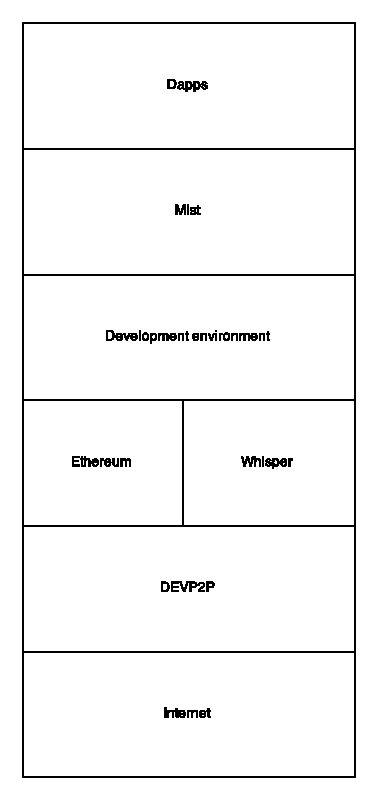
\includegraphics[width=0.30\linewidth]{figure/ethereum-applicationstack.pdf}
\centering
\caption{Ethereum Application Stack~\cite{eth:applicationstack}.
\textbf{TODO:} replace this with tikzpicture}
\end{figure}

Under the Ethereum umbrella project, a whole ecosystem for decentralized applications is developed. To interface decentralized applications to end users, the preffered method is to build front ends in standard web technologies, such as JavaScript and HTML, which most end users and developers are familiar with. Since the identity of the user is linked to their Ethereum public key, users never need to sign up or create accounts in these decentralized applications, since their public key uniquely identifies them.
From a development standpoint, this invites to rich client applications and thin servers. In figure 3.2, the application stack is listed. 

\section{Docker}
Software today is generally quite complex. A website, for example, is most often much more than a simple HTML-document. There might be a database, a server-side scripting engine (there are many), a few custom-built server-side programs for specific data processing or some common or uncommon software libraries. Since all pieces of work do not require all of these components, but may require other pieces of software instead, it is clearly both impractical and very limiting to bundle the required pieces of software as one large application stack. The best solution is to package each of these work-specific requirements (dependencies) together with the piece of work itself. A piece of software that accomplishes this goal is Docker.

\subsection{Virtualized containers}
Docker uses virtualization techniques to create isolated environments called containers, these can be executed as if they were a runnable file. How this is done is outside of the scope of this subject.
There are two distinct advantages for this; since the containers are a full application packaged with its dependencies, it comes pre-compiled and is ready to run on any architecture that supports Docker. 
The other advantage is that a piece of work is isolated from both the system it is running on, as well as other potential pieces of work. If the code were to run directly on the system a number of exploits would have been possible.~\cite{korpela:2012}

\subsection{Security}
An important factor when volunteering to run arbitrary code on your machine is security. 
How can you ensure that you are not running software that will read or corrupt the data on your disk. 
In an action to prevent this, Docker containers are executed in a separate environment, a \emph{kernel namespace}, to each other and the host machine. This means that it cannot know about or interact with the outside world~\cite{docker-security}. An application running totally isolated may not sound ideal for hosting a webapp, but that is where Docker shines again. You can specify ports where your application can be accessed from inside the virtual machine, thus again making it possible to run code in a secure way.
There are always security implications of running code not written by you, but we feel that we have done enough in the scope of this project.